\documentclass[a4paper,12pt]{article}
\usepackage[T1]{fontenc}
\usepackage{fullpage,graphicx,psfrag,amsmath,amsfonts}
\usepackage[small,bf]{caption}
\usepackage[utf8]{inputenc}
\usepackage[english]{babel}
\usepackage{lipsum}
\usepackage{url}
\usepackage{bm}
\usepackage{float}
\usepackage{kpfonts}
\usepackage{mathpazo}
\usepackage{enumitem}
\setitemize{noitemsep,topsep=0pt,parsep=0pt,partopsep=0pt}

\begin{document}
\author{Filippo Grotto VR460638}

\title{Physical Human Robot Interaction}

\maketitle
\tableofcontents

\section{Four channel bilateral teleoperation architecture}

\subsection{Continuous and discretized implementation}
Implement the SISO Four-channel bilateral teleoperation architecture with
\[
    C_m = B_m + \frac{K_m}{s} \quad
    C_s = B_s + \frac{K_s}{s}
\]
\[
    Z_m^{-1} = \frac{1}{M_ms + D_m} \quad
    Z_s^{-1} = \frac{1}{M_ss + D_s}
\]

\bigskip
\noindent where $Mm = 0.5$, $M_s = 2$. Moreover $D_s = 10$ and $D_m = 5$ or both zero in the initial case. In Fig \ref{fig:hw1} a simple plot of the positions and velocities (slave and master) are reported for proper selected tuning parameters of the related master and slave controller. In order to properly tune the controllers the following closed-loop systems were considered:

\[
G_m = \frac{1}{M_ms^2+B_ms+K_m} \quad
G_s = \frac{1}{M_ss^2+B_ss+K_s}
\]

\bigskip
\noindent The proper parameters were selected considering the step reponse of the two second order systems. For the human intention controller the parameters were selected by comparing the reference position with the master/slave position and perform proper tuning (an analytical closed-loop system might also be considered for this analysis).

\begin{figure}[H]
    \begin{center}
        \hspace*{-2cm}
        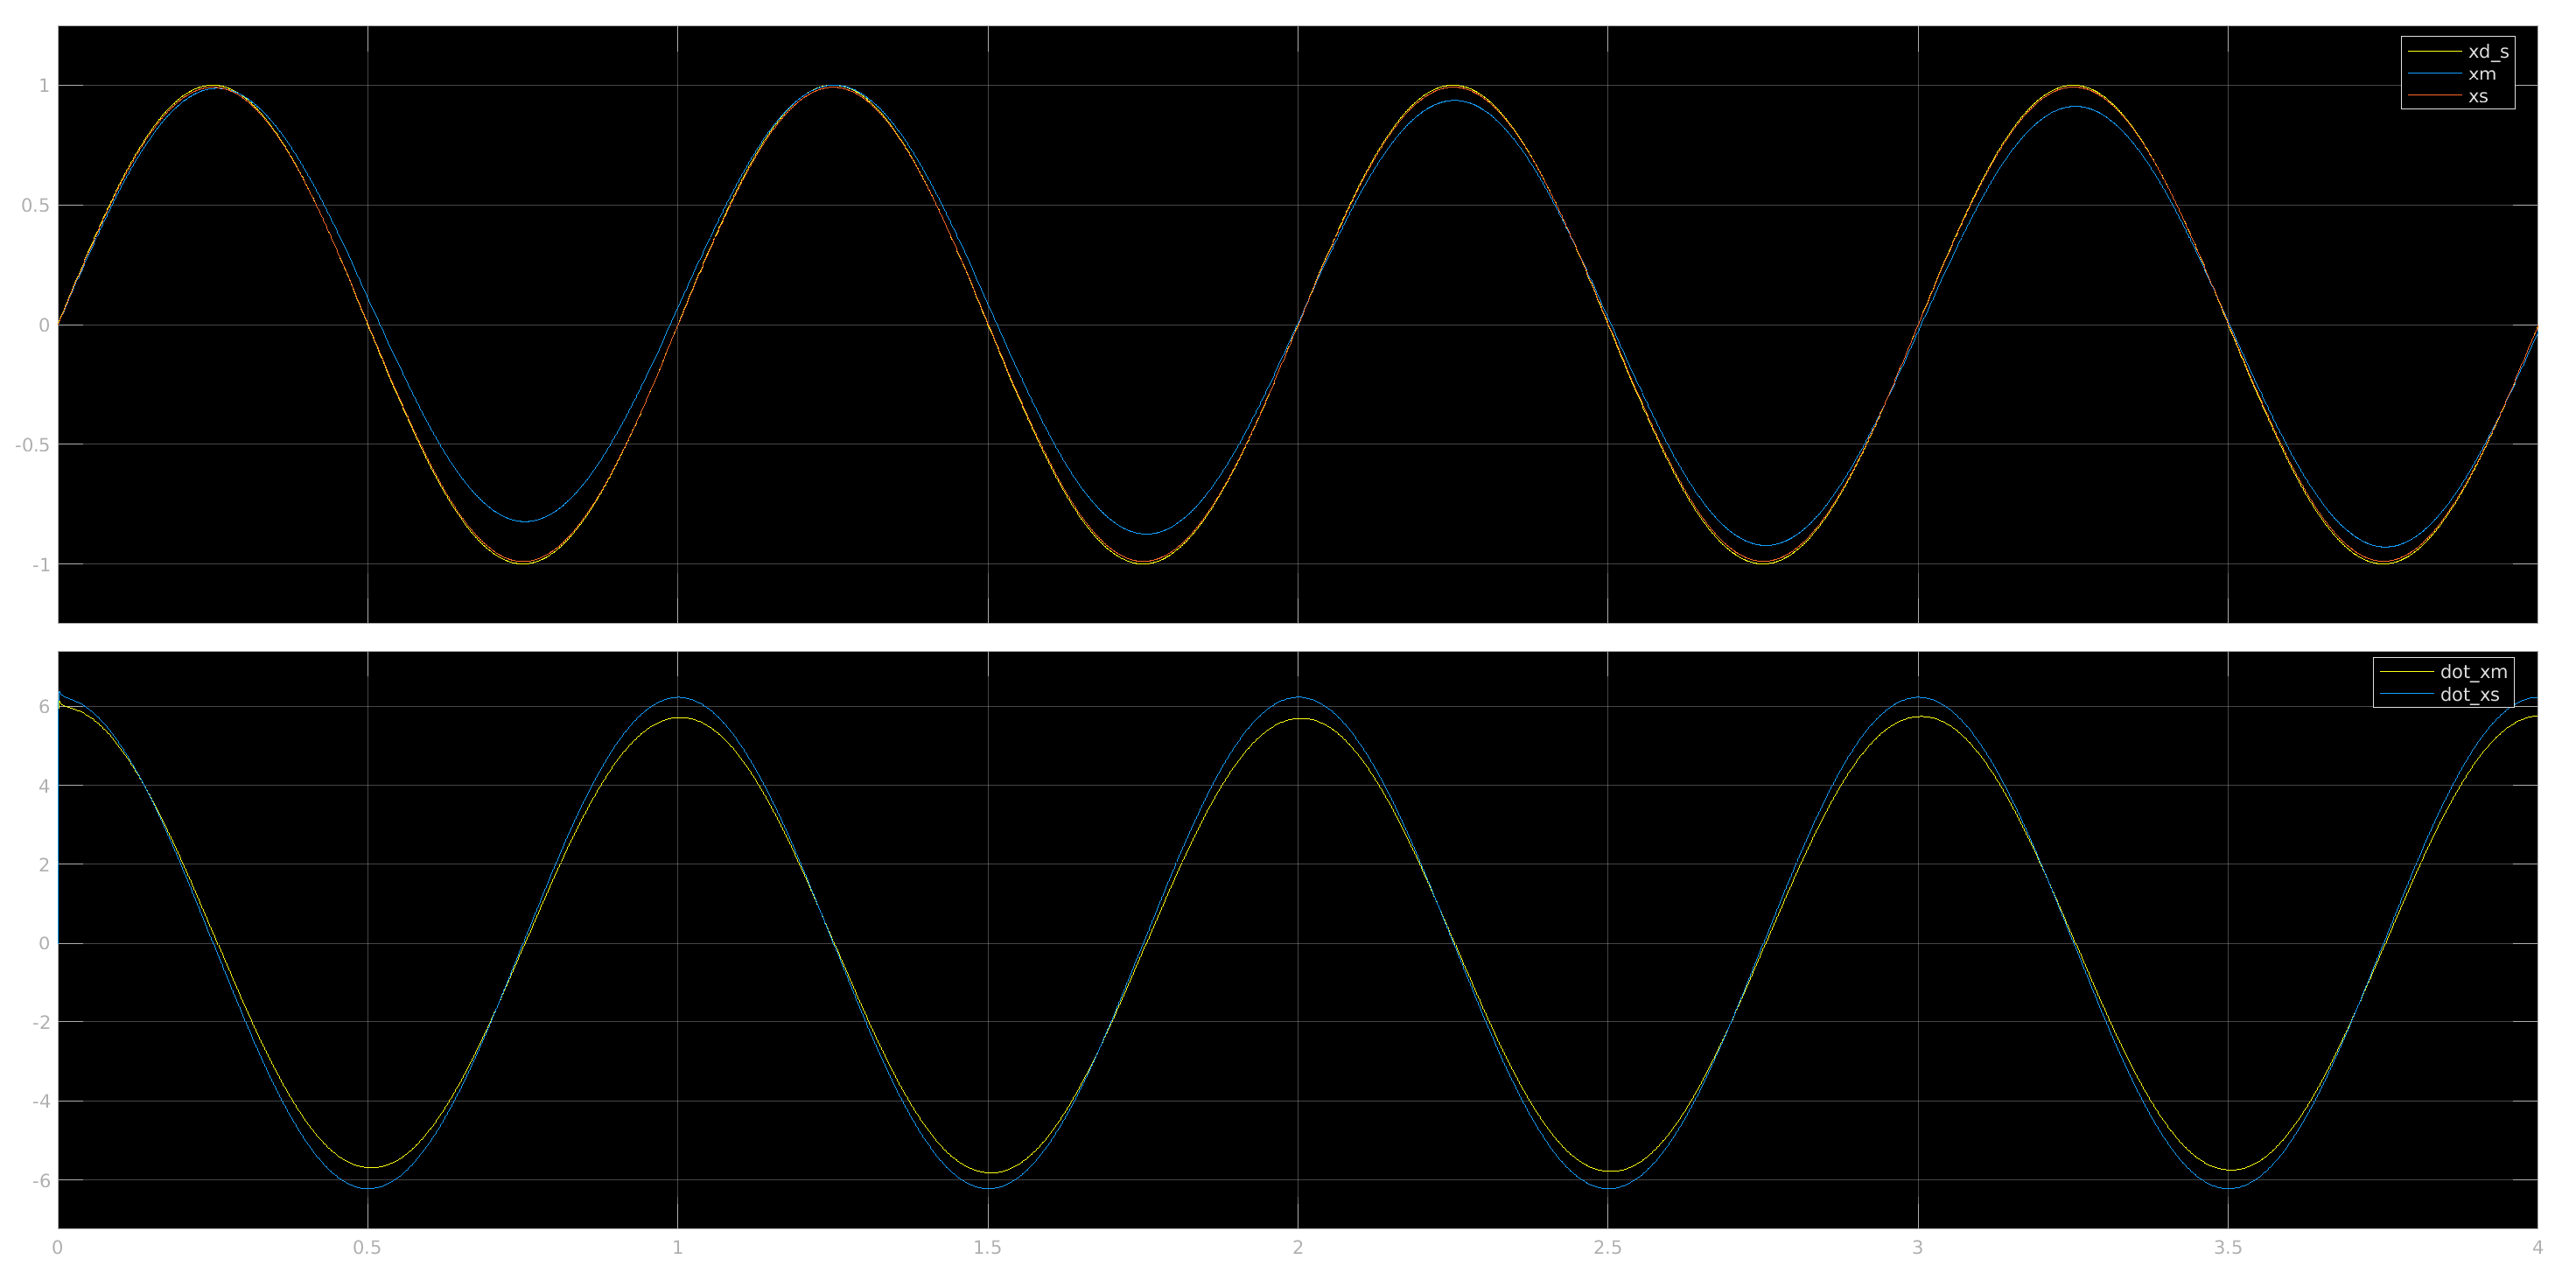
\includegraphics[scale=0.39]{images/hw1.eps}
    \end{center}
    \caption{Reference slave and master position are depicted in the first plot. Slave and Master velocities are reported in the second plot}
    \label{fig:hw1}
\end{figure}

\begin{figure}[H]
    \begin{center}
        \hspace*{-2cm}
        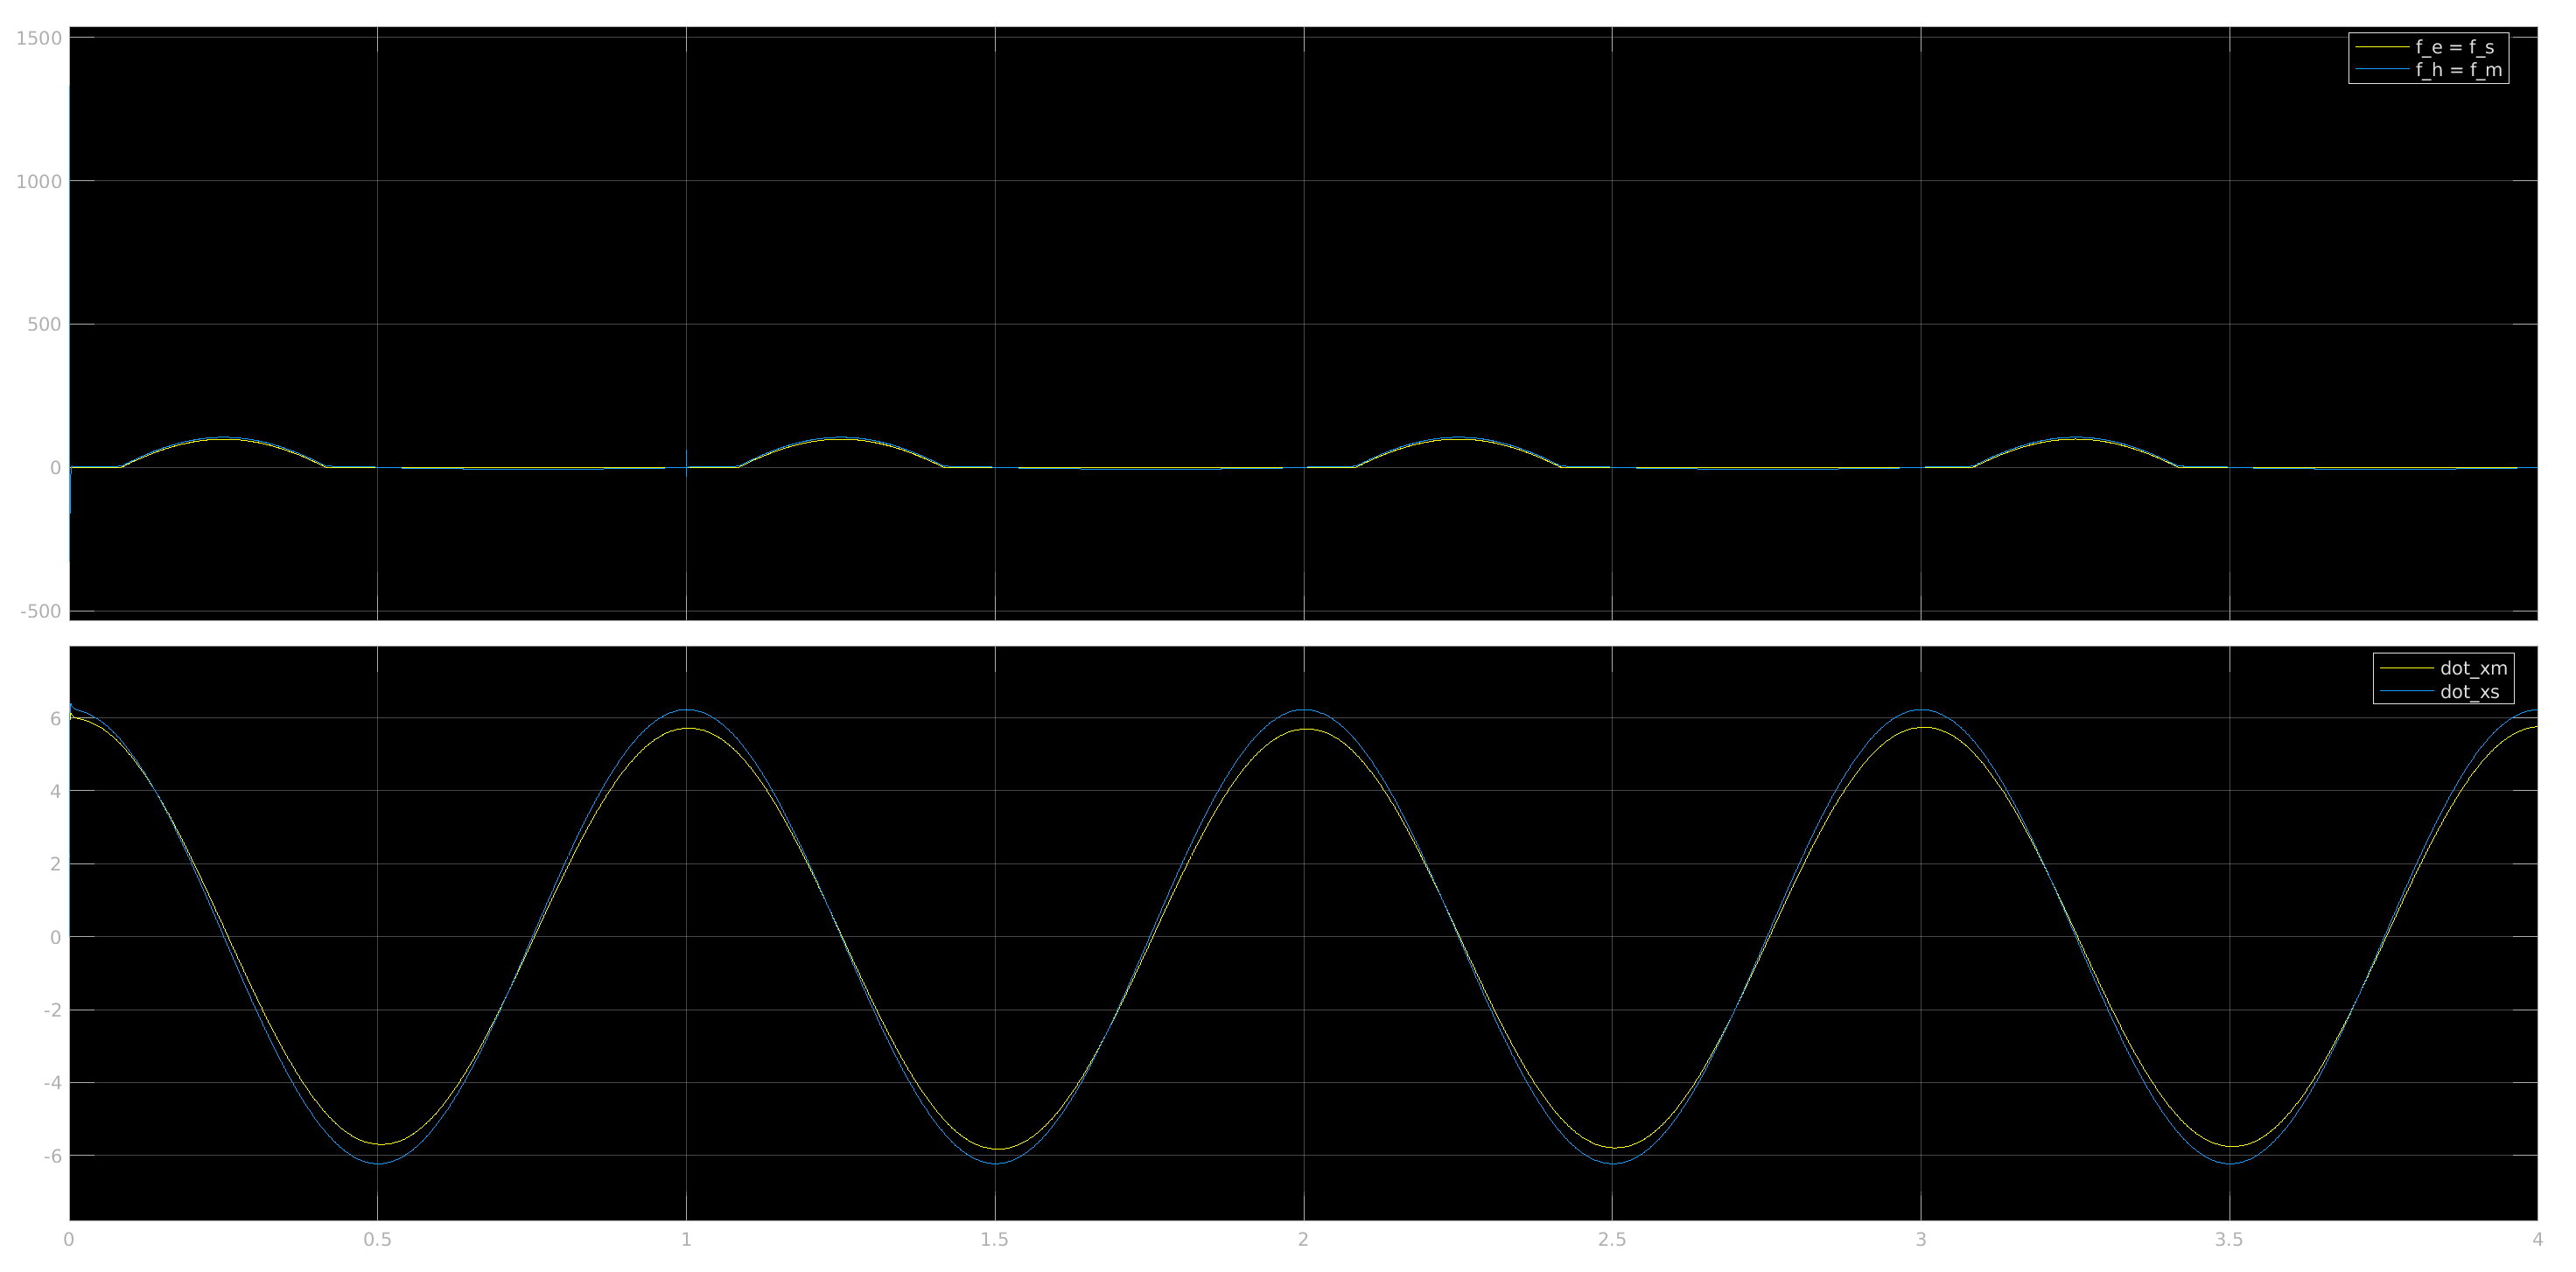
\includegraphics[scale=0.39]{images/hw1_forces.eps}
    \end{center}
    \caption{Master and slave velocity and forces compared when the environment is not attached to the end effector of the robot. The environment force has to be zero when not in contact}
    \label{fig:hw1_forces}
\end{figure}

\noindent Finally the entire architecture was translated in the related discretized version according to our specification in terms of encoders and the related derivative were performed using the simulink block. In the following section a proper estimation tool will be analysed.
    
\end{document}
